\let\negmedspace\undefined
\let\negthickspace\undefined
\documentclass[journal]{IEEEtran}
\usepackage[a4paper, margin=10mm, onecolumn]{geometry}
\usepackage{tfrupee}
\setlength{\headheight}{1cm}
\setlength{\headsep}{0mm}

\usepackage{gvv-book}
\usepackage{gvv}
\usepackage{cite}
\usepackage{amsmath,amssymb,amsfonts,amsthm}
\usepackage{algorithmic}
\usepackage{graphicx}
\usepackage{float}
\usepackage{textcomp}
\usepackage{xcolor}
\usepackage{txfonts}
\usepackage{listings}
\usepackage{enumitem}
\usepackage{mathtools}
\usepackage{gensymb}
\usepackage{comment}
\usepackage[breaklinks=true]{hyperref}
\usepackage{tkz-euclide}
\usepackage{listings}
\def\inputGnumericTable{}
\usepackage[latin1]{inputenc}
\usepackage{color}
\usepackage{array}
\usepackage{longtable}
\usepackage{calc}
\usepackage{multirow}
\usepackage{hhline}
\usepackage{ifthen}
\usepackage{lscape}
\usepackage{tikz}
\usetikzlibrary{patterns}

\begin{document}

\bibliographystyle{IEEEtran}
\vspace{3cm}

\title{8.2.33}
\author{EE25BTECH11065 - Yoshita J}

{\let\newpage\relax\maketitle}

\renewcommand{\thefigure}{\theenumi}
\renewcommand{\thetable}{\theenumi}
\setlength{\intextsep}{10pt}

\textbf{Question}\\
Find the equation of the conic with length of major axis $26$, foci $\brak{\pm 5,0}$.\\

\textbf{Solution}\\
The equation of a conic is
\begin{align}
\vec{x}^T V \vec{x} + 2\vec{u}^T \vec{x} + f = 0 \tag{1}
\end{align}
where
\begin{align}
V = \|\vec{n}\|^2 I - e^2\vec{n}\vec{n}^T \tag{2}
\end{align}

The foci are
\begin{align}
\vec{F}_1 = \myvec{5\\0},\quad \vec{F}_2 = \myvec{-5\\0} \tag{3}
\end{align}

The centre is
\begin{align}
\vec{u} = \frac{\vec{F}_1+\vec{F}_2}{2} = \myvec{0\\0} \tag{4}
\end{align}

The axis vector is
\begin{align}
\vec{n} = \vec{F}_1-\vec{F}_2 = \myvec{1\\0} \tag{5}
\end{align}

Therefore, substituting $\vec{n}=\myvec{1\\0}$ in (2), we get
\begin{align}
V = \myvec{1-e^2 & 0 \\ 0 & 1} \tag{6}
\end{align}

From the formula for the length of the major axis,
\begin{align}
2\sqrt{\frac{|f|}{\lambda_1}} \tag{7}
\end{align}
where $\lambda_1 = 1-e^2$. Hence
\begin{align}
26 = 2\sqrt{\frac{|f|}{1-e^2}} \tag{8}
\end{align}

The relation between focus and eccentricity is
\begin{align}
\pm ce^2 = 5 \tag{9}
\end{align}

The distance $c$ is
\begin{align}
c = \pm \frac{1}{e}\sqrt{\frac{|f|}{|e^2-1|}} \tag{10}
\end{align}

Thus from (8)--(10), solving the unknowns $(c,e,f)$ we get
\begin{align}
e = \tfrac{5}{13},\quad c = \pm 5, \quad |f| = 144. \tag{11}
\end{align}

Let $\vec{x}=\myvec{0\\\alpha}$ be a vertex on the minor axis. Substituting in (1):
\begin{align}
\frac{12^2}{1} + f = 0 \implies f=-144. \tag{12}
\end{align}

Hence the equation of the conic is
\begin{align*}
\vec{x}^T \myvec{\tfrac{144}{169} & 0 \\ 0 & 1} \vec{x} - 144 = 0. \tag{13}
\end{align*}

\begin{figure}[H]
    \centering
    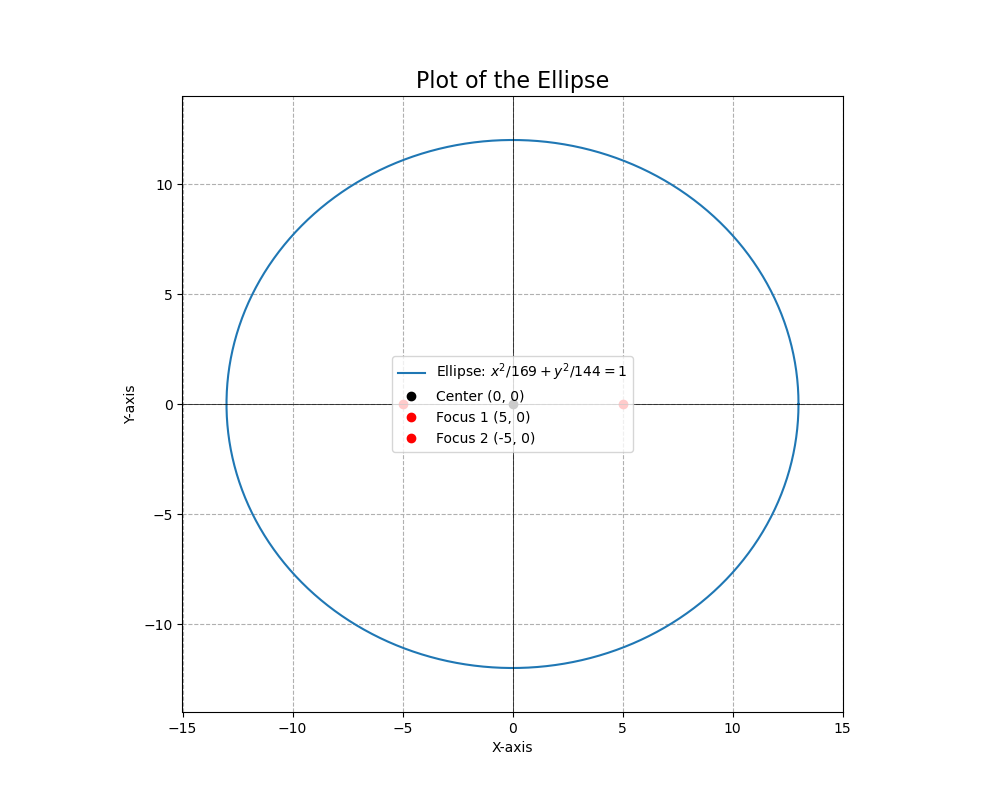
\includegraphics[width=0.9\linewidth]{figs/fig3.png}
    \caption{Ellipse with major axis $26$ and foci at $(\pm 5,0)$}
    \label{fig:ellipse}
\end{figure}

\end{document}

